\documentclass[12pt]{report}
\usepackage{graphicx} % Required for inserting images
\usepackage[a4paper, margin=2.5cm]{geometry}
\graphicspath{{images/}}

\usepackage[utf8]{inputenc}
\usepackage[T1]{fontenc}
\usepackage{float} % here for H placement parameter
\usepackage{subcaption}

\usepackage{filecontents}
\usepackage[
    firstinits=true, % render first and middle names as initials
    useprefix=true,
    maxcitenames=3,
    maxbibnames=99,
    style=authoryear,
    dashed=false, % re-print recurring author names in bibliography
    natbib=true,
    url=false
]{biblatex}

\title{CMP5352 Report - TITLE NEEDED}
\author{Lewis Higgins - Student ID 22133848}
\date{April 2024}

\usepackage[outputdir=./auxil]{minted}

\renewbibmacro*{volume+number+eid}{%
    \printfield{volume}%
%  \setunit*{\adddot}% DELETED
    \setunit*{\addnbspace}% NEW (optional); there's also \addnbthinspace
    \printfield{number}%
    \setunit{\addcomma\space}%
    \printfield{eid}}
\DeclareFieldFormat[article]{number}{\mkbibparens{#1}}

\addbibresource{report.bib}

% Use single quotes around titles:
\usepackage[british]{babel}
\usepackage{csquotes}

\usepackage{hyperref}

\hypersetup{
    colorlinks=true,
    linkcolor=black,
    filecolor=magenta,
    urlcolor=blue,
    citecolor=black,
}


\urlstyle{same}


% To prevent "Chapter N" display for each chapter
\usepackage[compact]{titlesec}
\usepackage{wasysym}
\usepackage{import}

\titlespacing*{\chapter}{0pt}{-2cm}{0.5cm}
\titleformat{\chapter}[display]
{\normalfont\bfseries}{}{0pt}{\Huge}

\newcommand\blfootnote[1]{
    \begingroup
    \renewcommand\thefootnote{}\footnote{#1}
    \addtocounter{footnote}{-1}
    \endgroup
}

\usepackage{fancyhdr}
\usepackage{calc}
\pagestyle{fancy}

\setlength\headheight{37pt}

\renewcommand{\chaptermark}[1]{%
    \markboth{#1}{}}

\lhead{Lewis Higgins - ID 22133848~~~~~~~~~~~~~~~
\includegraphics[width=1.75cm]{bcu logo}}
\fancyhead[R]{\leftmark}

\usepackage{xcolor}
\definecolor{mintedBG}{rgb}{0.95, 0.95, 0.95}

\begin{document}
    \pagecolor{yellow} % Change in final

    \makeatletter
    \begin{titlepage}
        \begin{center}
            
\includegraphics[width=0.7\linewidth]{bcu logo}\\[4ex]
            {\large \bfseries  \@title }\\[2ex]
            {\large \bfseries  DRAFT VERSION }\\[2ex]
            {\@author}\\[30ex]
            {Word count: XXXX}\\[20ex]
        \end{center}
    \end{titlepage}
    \makeatother
    \thispagestyle{empty}
    \newpage

    \pagecolor{white}

    \begin{abstract}
        text

        text

        text

    \end{abstract}

    \setcounter{page}{0} % Page counter bullshit to make it ACTUALLY start from 1

    \tableofcontents
    \thispagestyle{empty}

    \chapter*{Introduction}\label{ch:introduction}
    \addcontentsline{toc}{chapter}{Introduction}
    \markboth{Introduction}{}

    Text text text

    Text text text

    \pagebreak

    aaa

    \chapter*{Motivation and objectives}\label{ch:sec1}
    \addcontentsline{toc}{chapter}{Motivation and objectives}
    \markboth{Motivation and objectives}{}


%   \inputminted[linenos=true, breaklines=true, bgcolor=mintedBG, stripall=true]{r}{lab4.R}
    \begin{minted}[]{r}
library(ggplot2)

# Side-note that if you run this as a file and not in the IDE the plots will
# actually be put into a PDF for you in the active working directory (here).

# We can use a randomly selected sample of the dataset for the graph.
# However, because the results should be reproducible, we should set an RNG seed.
set.seed(1000)

# Select the numbered rows of the numbers produced by sample.
# Sample picks 100 random numbers.
dsmall <- diamonds[sample(nrow(diamonds), 100),]
# The random comma at the end tells R that you're slecting ROWS, not columns.
# If you don't put this comma it assumes you're looking to select the columns.

qplot(log(carat), log(price), data = dsmall, geom = "smooth")
\end{minted}

\begin{minted}[]{text}
## `geom_smooth()` using method = 'loess' and formula = 'y ~ x'
\end{minted}

\begin{figure}[H]

{\centering 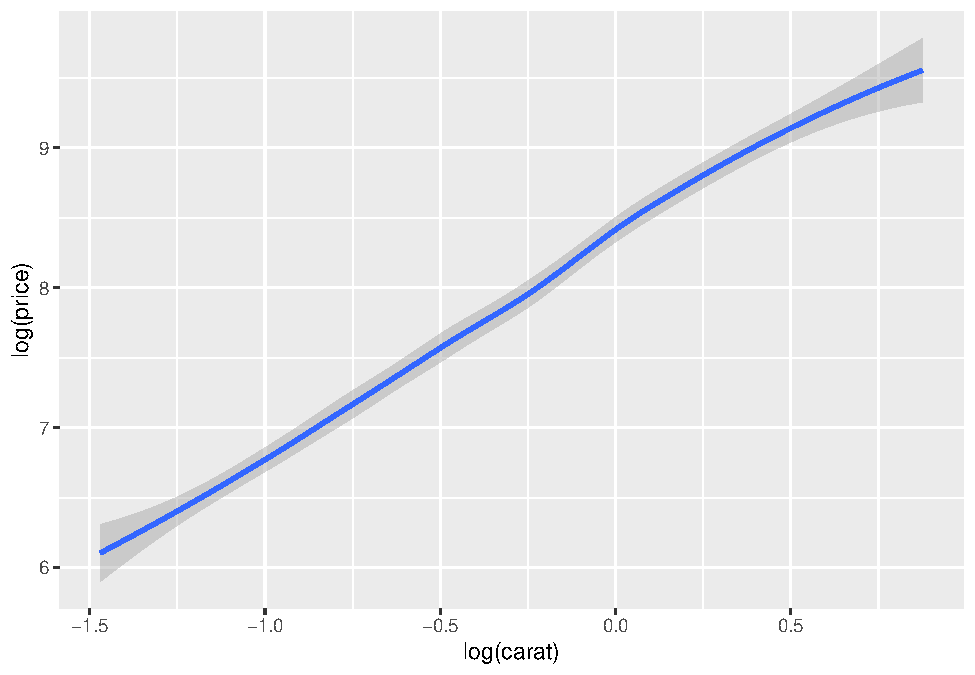
\includegraphics[width=0.75\linewidth]{C:/Users/Lewis/DataspellProjects/DataVis/Assignment/LaTeX/RMD/test2_files/figure-latex/unnamed-chunk-2-1} 

}

\caption{Figure AAA}\label{fig:unnamed-chunk-2-1}
\end{figure}

\begin{minted}[]{r}
# Can supply multiple geoms in a vector
qplot(log(carat), log(price), data = dsmall, geom = c("point", "smooth"))
\end{minted}

\begin{minted}[]{text}
## `geom_smooth()` using method = 'loess' and formula = 'y ~ x'
\end{minted}

\begin{figure}[H]

{\centering 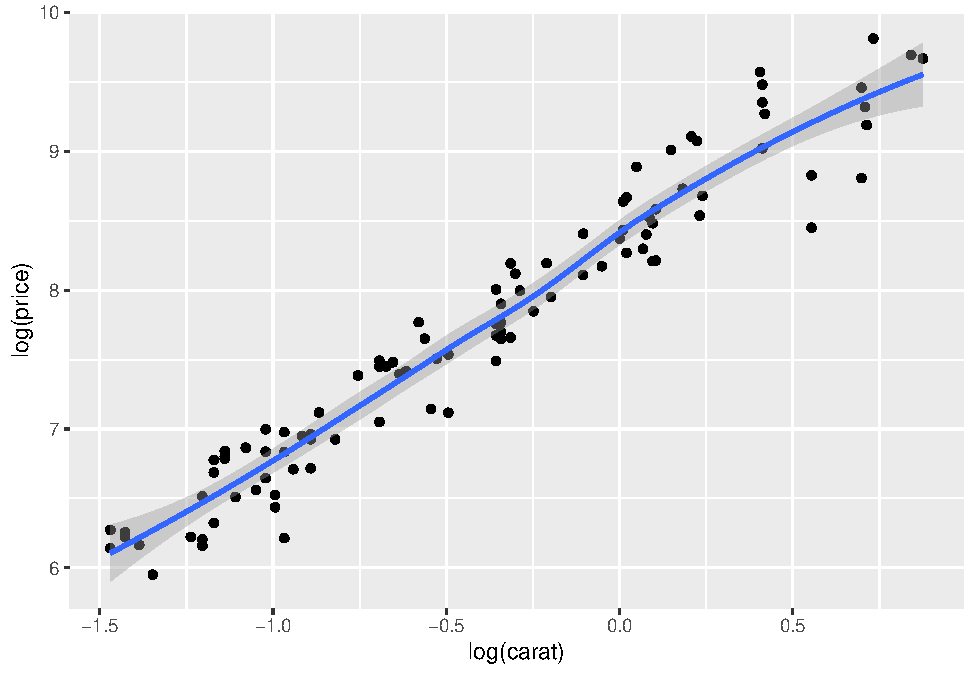
\includegraphics[width=0.75\linewidth]{C:/Users/Lewis/DataspellProjects/DataVis/Assignment/LaTeX/RMD/test2_files/figure-latex/unnamed-chunk-2-2} 

}

\caption{Figure AAA}\label{fig:unnamed-chunk-2-2}
\end{figure}

\begin{minted}[]{r}
# Different smooth line?

# Span varies the smoothness of geom_smooth from 0 to 1 where 1 is the smoothest.
# It states that span is an unknown parameter, yet this does actually
# modify the produced graph. 0.2 is the minimum before R throws warnings.
# 0.1 works with warnings, but anything lower produces no smooth line.
# Though, using 0.1 means you might as well not even put a smooth line.
qplot(log(carat), log(price), data = dsmall, geom = c("point", "smooth"), span = 0.2)
\end{minted}

\begin{minted}[]{text}
## `geom_smooth()` using method = 'loess' and formula = 'y ~ x'
\end{minted}

\begin{figure}[H]

{\centering 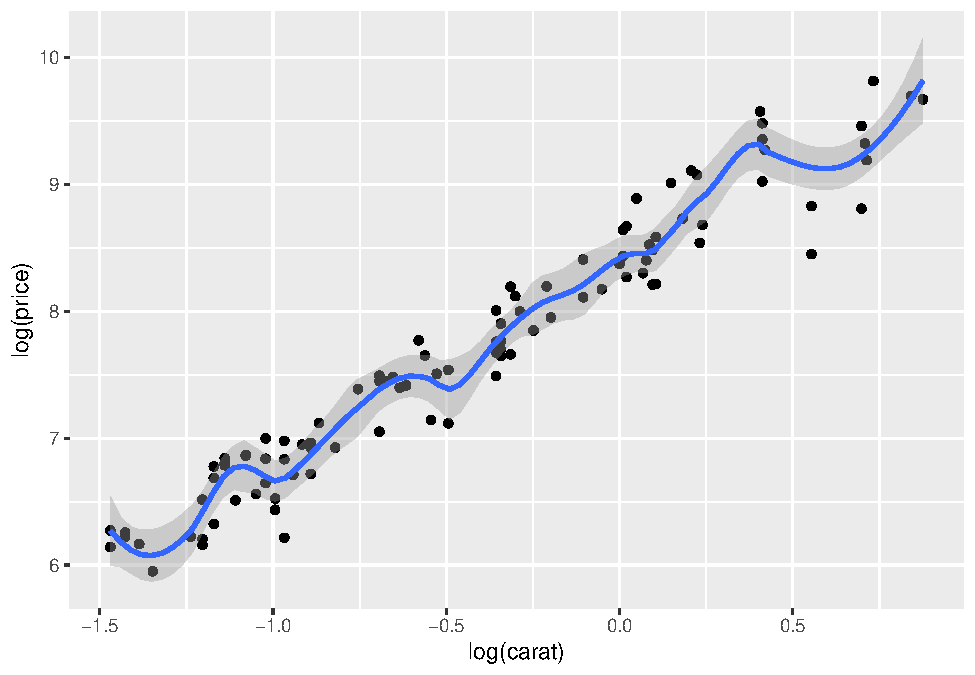
\includegraphics[width=0.75\linewidth]{C:/Users/Lewis/DataspellProjects/DataVis/Assignment/LaTeX/RMD/test2_files/figure-latex/unnamed-chunk-2-3} 

}

\caption{Figure AAA}\label{fig:unnamed-chunk-2-3}
\end{figure}

\begin{minted}[]{r}
# You can also fit a linear model to the graph via lm.
qplot(log(carat), log(price), data = dsmall, geom = c("point", "smooth"), method = "lm")
\end{minted}

\begin{minted}[]{text}
## `geom_smooth()` using formula = 'y ~ x'
\end{minted}

\begin{figure}[H]

{\centering 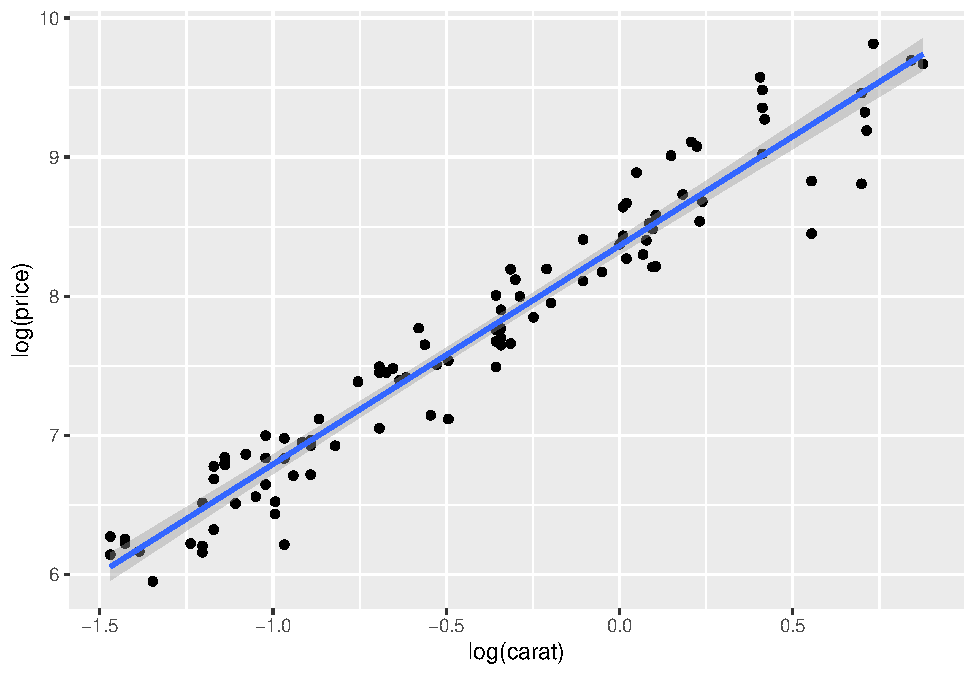
\includegraphics[width=0.75\linewidth]{C:/Users/Lewis/DataspellProjects/DataVis/Assignment/LaTeX/RMD/test2_files/figure-latex/unnamed-chunk-2-4} 

}

\caption{Figure AAA}\label{fig:unnamed-chunk-2-4}
\end{figure}

\begin{minted}[]{r}
# Scatterplotting a different dataset, ggplot's builtin mpg (car fuel economy data)
qplot(displ, hwy, data = mpg, color = drv)
\end{minted}

\begin{figure}[H]

{\centering 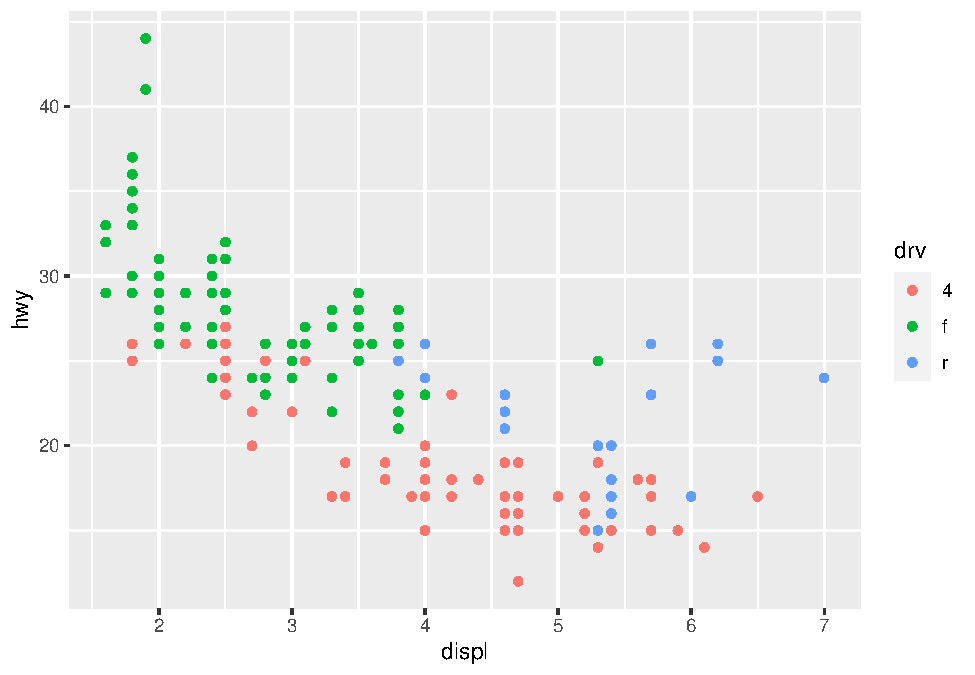
\includegraphics[width=0.75\linewidth]{C:/Users/Lewis/DataspellProjects/DataVis/Assignment/LaTeX/RMD/test2_files/figure-latex/unnamed-chunk-2-5} 

}

\caption{Figure AAA}\label{fig:unnamed-chunk-2-5}
\end{figure}

\begin{minted}[]{r}
# If you provided a color argument to this, it would draw one smooth for every color.
qplot(displ, hwy, data = mpg, geom = c("point", "smooth"))
\end{minted}

\begin{minted}[]{text}
## `geom_smooth()` using method = 'loess' and formula = 'y ~ x'
\end{minted}

\begin{figure}[H]

{\centering 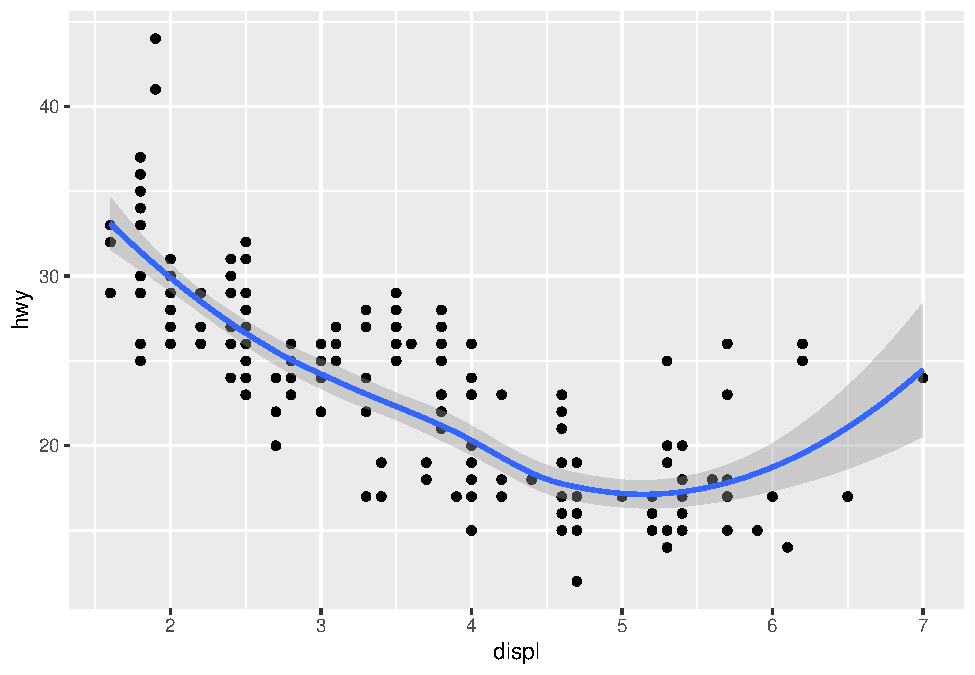
\includegraphics[width=0.75\linewidth]{C:/Users/Lewis/DataspellProjects/DataVis/Assignment/LaTeX/RMD/test2_files/figure-latex/unnamed-chunk-2-6} 

}

\caption{Figure AAA}\label{fig:unnamed-chunk-2-6}
\end{figure}

\begin{minted}[]{r}
# Answers the question "How are engine size and fuel economy related?"
# Turning cylinder into a factor (categorical data).
# Basically counts the appearances of each value.
qplot(displ, hwy, data = mpg, color = factor(cyl))
\end{minted}

\begin{figure}[H]

{\centering 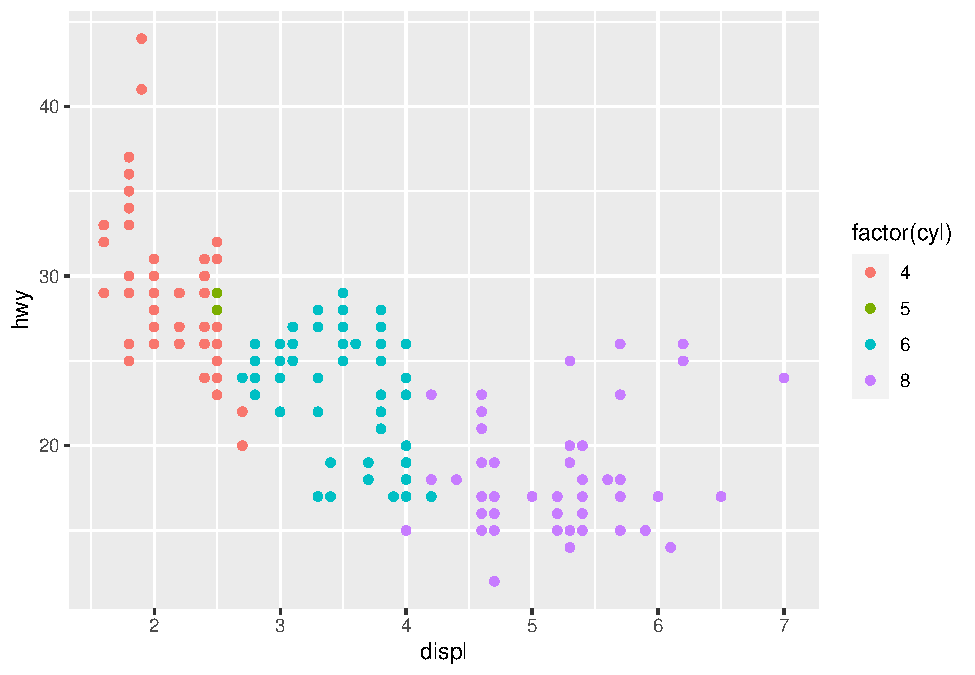
\includegraphics[width=0.75\linewidth]{C:/Users/Lewis/DataspellProjects/DataVis/Assignment/LaTeX/RMD/test2_files/figure-latex/unnamed-chunk-2-7} 

}

\caption{Figure AAA}\label{fig:unnamed-chunk-2-7}
\end{figure}

\begin{minted}[]{r}
# We can use all arguments previously shown at once.
# Note that there aren't enough 5 cylinders to fit a line, so there isn't one.
qplot(displ, hwy, data = mpg, color = factor(cyl),
      geom = c("point", "smooth"), method = "lm")
\end{minted}

\begin{minted}[]{text}
## `geom_smooth()` using formula = 'y ~ x'
\end{minted}

\begin{figure}[H]

{\centering 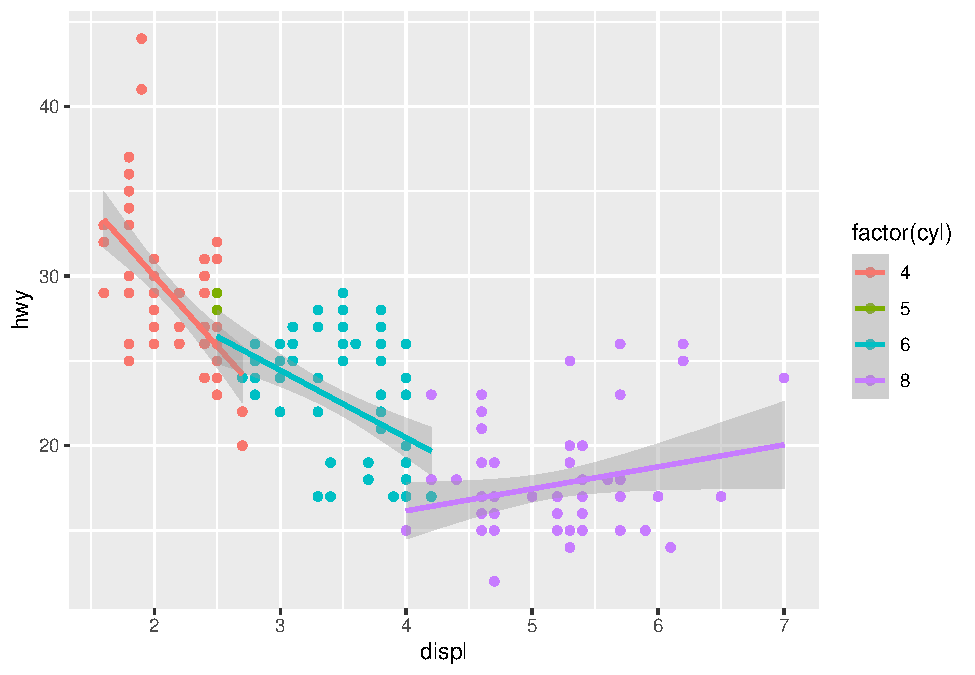
\includegraphics[width=0.75\linewidth]{C:/Users/Lewis/DataspellProjects/DataVis/Assignment/LaTeX/RMD/test2_files/figure-latex/unnamed-chunk-2-8} 

}

\caption{Figure AAA}\label{fig:unnamed-chunk-2-8}
\end{figure}

\begin{minted}[]{r}
### --- Faceting --- ###


# . acts as a placeholder, indicating that there's no variable.
# Results in three seperate histograms, one of each drive class.
qplot(hwy, data = mpg, facets = drv ~ ., binwidth = 2)
\end{minted}

\begin{figure}[H]

{\centering 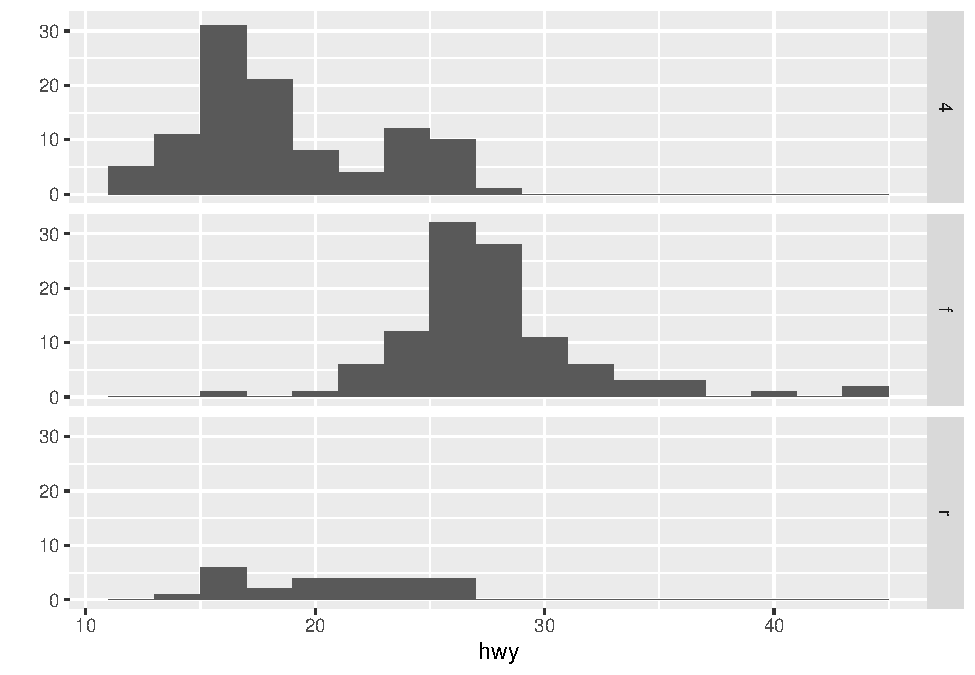
\includegraphics[width=0.75\linewidth]{C:/Users/Lewis/DataspellProjects/DataVis/Assignment/LaTeX/RMD/test2_files/figure-latex/unnamed-chunk-2-9} 

}

\caption{Figure AAA}\label{fig:unnamed-chunk-2-9}
\end{figure}

\begin{minted}[]{r}
# Could add colors. Doesn't help much though.

# Flips sideways. displ is displacement. Air movement per engine rev possibly
qplot(displ, hwy, data = mpg, facets = . ~ drv, geom = c("point", "smooth"))
\end{minted}

\begin{minted}[]{text}
## `geom_smooth()` using method = 'loess' and formula = 'y ~ x'
\end{minted}

\begin{figure}[H]

{\centering 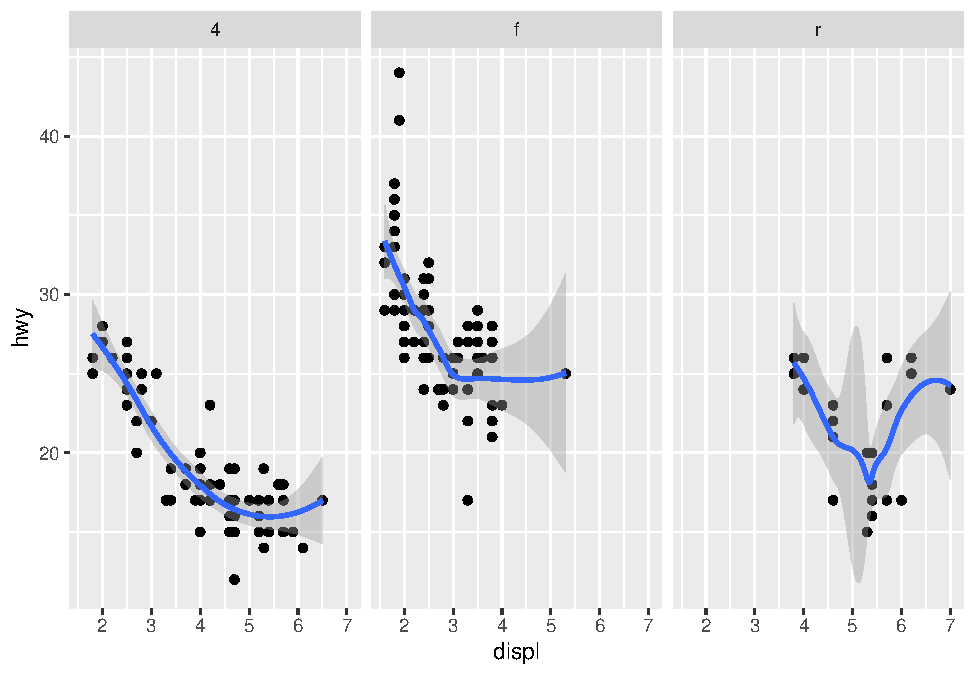
\includegraphics[width=0.75\linewidth]{C:/Users/Lewis/DataspellProjects/DataVis/Assignment/LaTeX/RMD/test2_files/figure-latex/unnamed-chunk-2-10} 

}

\caption{Figure AAA}\label{fig:unnamed-chunk-2-10}
\end{figure}

\begin{minted}[]{r}
# Reusing the diamond set.
qplot(carat, data = diamonds, facets = color ~ ., geom = "histogram")
\end{minted}

\begin{minted}[]{text}
## `stat_bin()` using `bins = 30`. Pick better value with `binwidth`.
\end{minted}

\begin{figure}[H]

{\centering 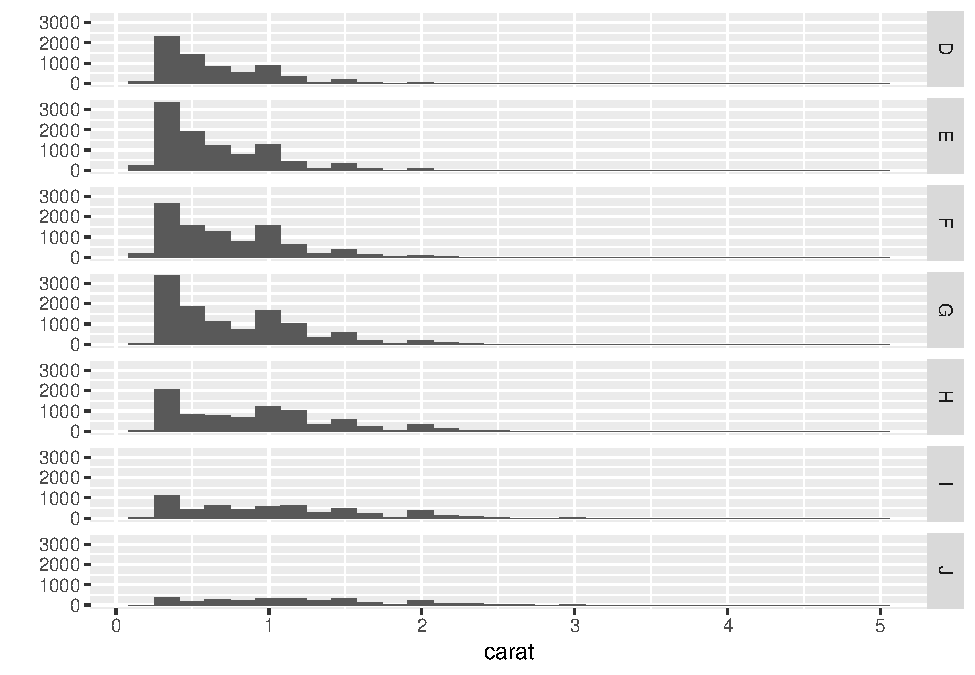
\includegraphics[width=0.75\linewidth]{C:/Users/Lewis/DataspellProjects/DataVis/Assignment/LaTeX/RMD/test2_files/figure-latex/unnamed-chunk-2-11} 

}

\caption{Figure AAA}\label{fig:unnamed-chunk-2-11}
\end{figure}

\begin{minted}[]{r}
# ..density.. tells ggplot to map the density as the Y-axis, instead of just counting.
qplot(carat, ..density.., data = diamonds, facets = color ~ ., geom = "histogram")
\end{minted}

\begin{minted}[]{text}
## `stat_bin()` using `bins = 30`. Pick better value with `binwidth`.
\end{minted}

\begin{figure}[H]

{\centering 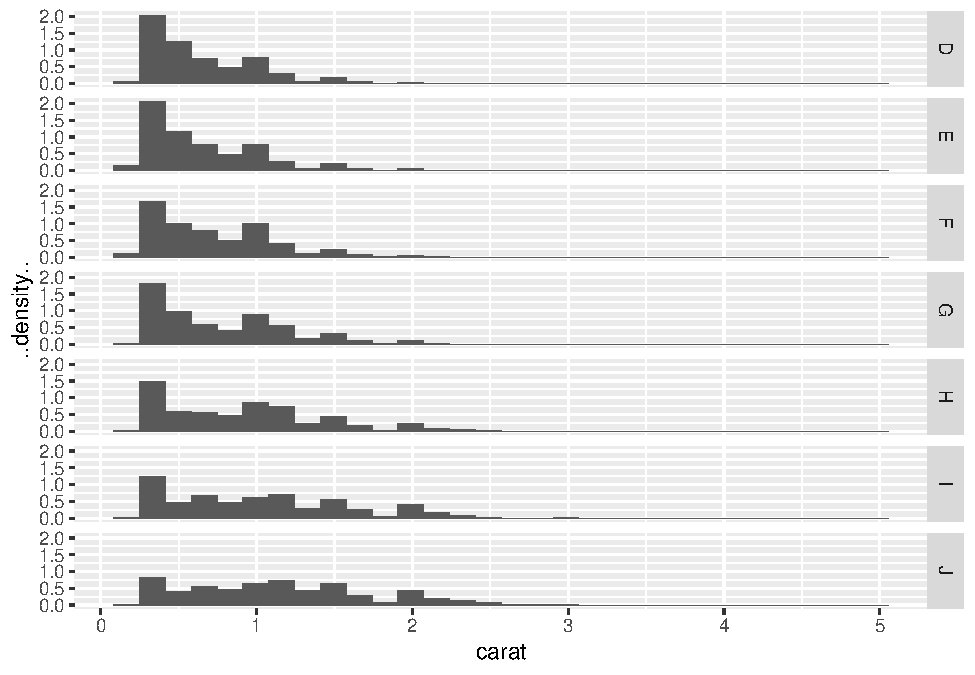
\includegraphics[width=0.75\linewidth]{C:/Users/Lewis/DataspellProjects/DataVis/Assignment/LaTeX/RMD/test2_files/figure-latex/unnamed-chunk-2-12} 

}

\caption{Figure AAA}\label{fig:unnamed-chunk-2-12}
\end{figure}

\begin{minted}[]{r}
# Plots thirty five histograms by also grouping by cut.
qplot(carat, data = diamonds, facets = color ~ cut, geom = "histogram")
\end{minted}

\begin{minted}[]{text}
## `stat_bin()` using `bins = 30`. Pick better value with `binwidth`.
\end{minted}

\begin{figure}[H]

{\centering 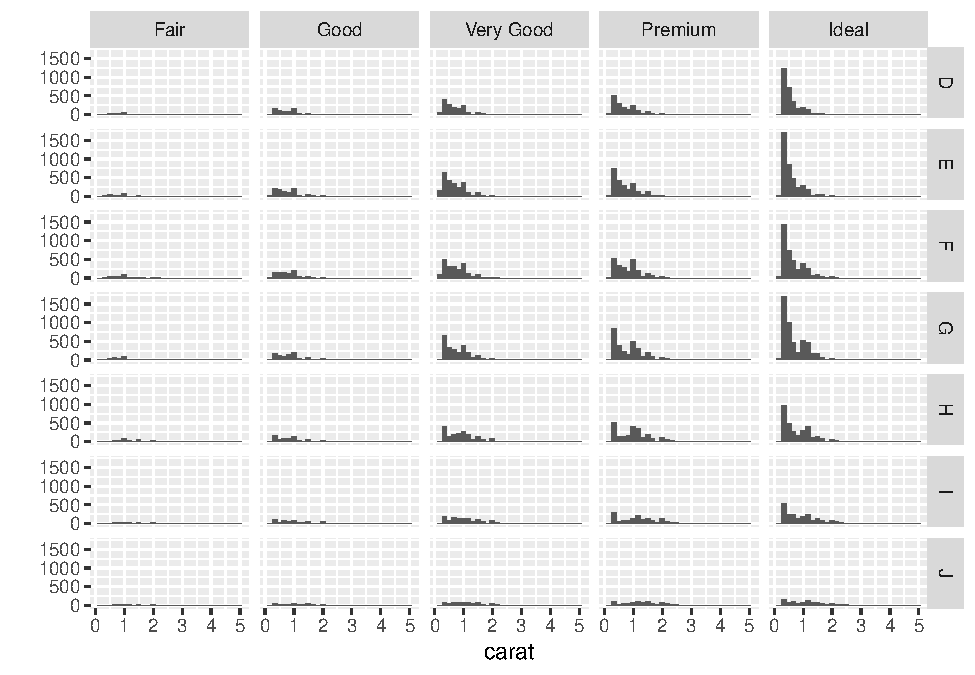
\includegraphics[width=0.75\linewidth]{C:/Users/Lewis/DataspellProjects/DataVis/Assignment/LaTeX/RMD/test2_files/figure-latex/unnamed-chunk-2-13} 

}

\caption{Figure AAA}\label{fig:unnamed-chunk-2-13}
\end{figure}
\begin{figure}

\includegraphics[width=0.5\linewidth]{../images/bcu logo} \caption{A nice image.}\label{fig:unnamed-chunk-3}
\end{figure}


    \pagebreak


    \chapter*{Experimental results}\label{ch:sec2}
    \addcontentsline{toc}{chapter}{Experimental results}
    \markboth{Experimental results}{}

    text text text

text text text

    \chapter*{Summary \& conclusion}\label{ch:sec3}
    \addcontentsline{toc}{chapter}{Summary and conclusion}
    \markboth{Summary and conclusion}{}

    text text text

text text text


\end{document}